\chapter{रासायनिक साम्य: भागफल और स्थिरांक}\label{ch:g12:equilibrium}

सोडा-पानी की बंद बोतल महीनों तक अपनी फ़िज़ बनाए रखती है; खुलने पर
वह एक दोपहर में बेदम हो जाती है। दोनों में से किसी भी स्थिति में कुछ गड़बड़ नहीं हुई है।
बंद बोतल में कार्बन डाइऑक्साइड पानी छोड़ती है और उसी दर से
उसमें लौटती है, और संरचना जस की तस रहती है; ढक्कन खोलिए, और जो गैस
निकलती है वह अब लौटती नहीं। अनेक अभिक्रियाएँ ऐसा ही व्यवहार करती हैं: वे
किसी भी \omterm{def:g7:chemical-reactions:reactant}{अभिकारक} के खपने से पहले रुक जाती हैं, दो विपरीत अभिक्रियाओं के
संतुलन पर। यह अध्याय उस संतुलन का वर्णन एक संख्या से करता है।

\begin{recall}
किसी \omterm{def:g10:reaction-progress-table:extent}{अभिक्रिया की प्रगति} $x$, उसका अधिकतम $x_{\max}$, और वे \omterm{def:g10:reaction-progress-table:limiting}{पूर्ण
अभिक्रियाएँ} जो उस तक पहुँचती हैं (\cref{ch:g10:reaction-progress-table})। दरें और
\omterm{def:g12:reaction-rates:kinetic-factor}{गतिक कारक} (\cref{ch:g12:reaction-rates}); \omterm{def:g12:catalysis:catalyst}{उत्प्रेरक}
\omterm{def:g10:reaction-progress-table:system}{अंतिम अवस्था} नहीं बदलता (\cref{ch:g12:catalysis})।
\end{recall}

\begin{omfigure}
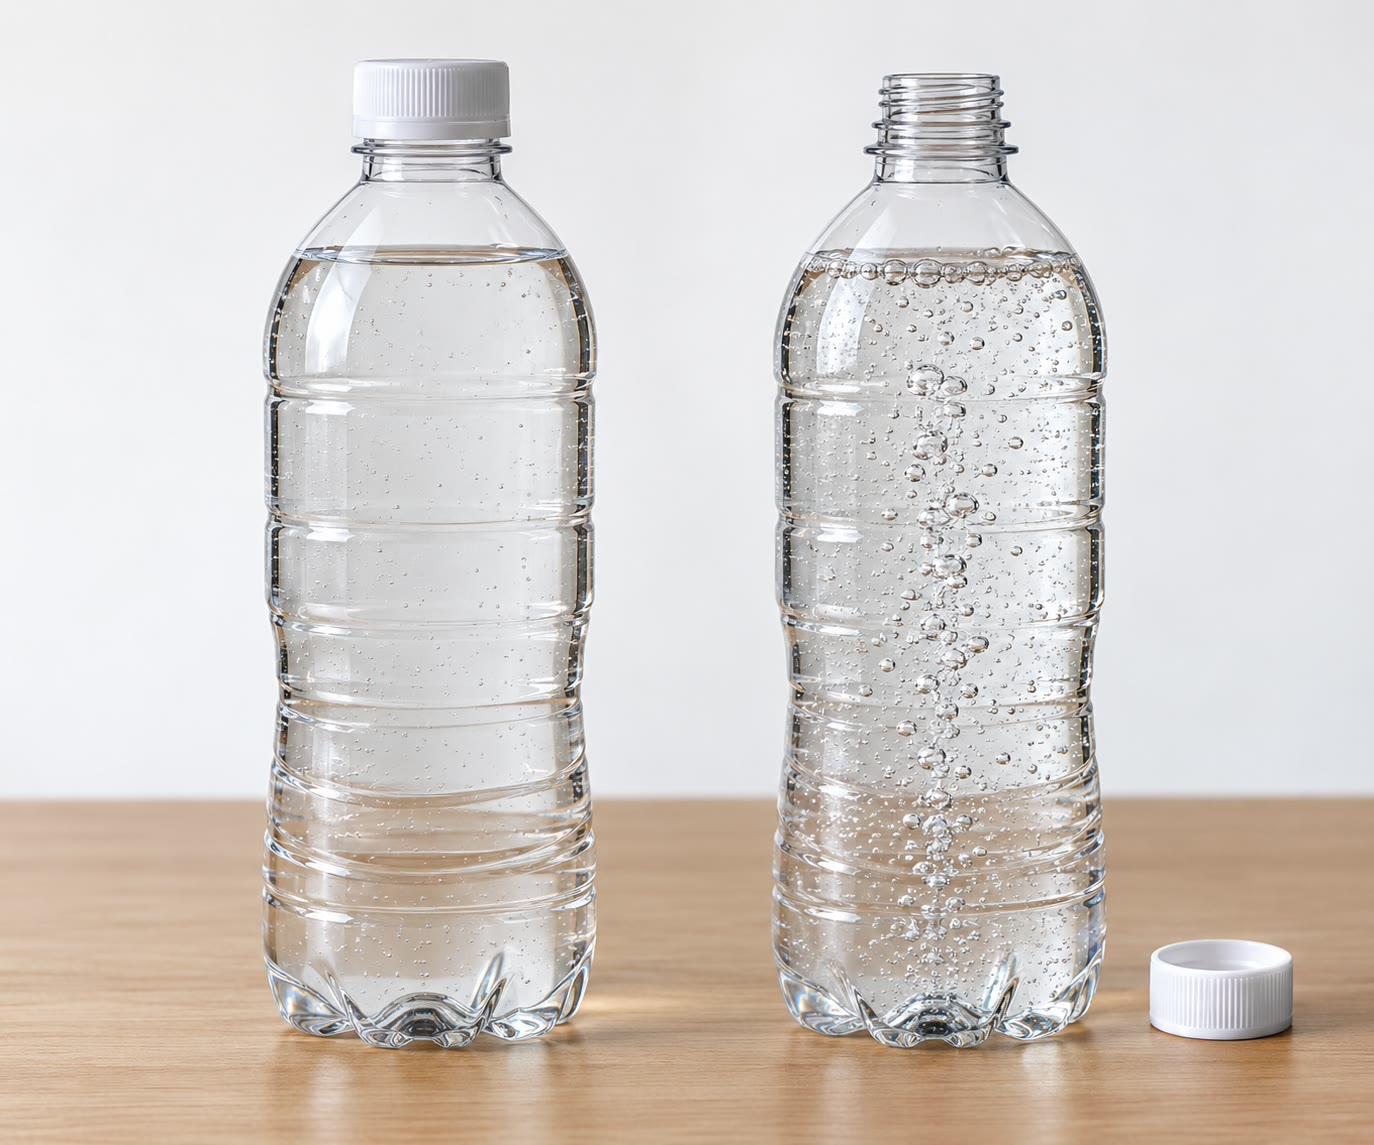
\includegraphics[width=0.45\linewidth,height=5cm,keepaspectratio]{images/book1/ai/g12-fizzy-bottles.jpg}

{\small बंद रहने पर पानी अपनी गैस बनाए रखता है; खुलने पर गैस निकल जाती है और
लौटती नहीं।}
\end{omfigure}

\section{वे अभिक्रियाएँ जो पूर्ण नहीं होतीं}

\begin{definition}[अपूर्ण अभिक्रिया, अंतिम प्रगति अनुपात]\label{def:g12:equilibrium:non-total}
कोई अभिक्रिया \emph{अपूर्ण अभिक्रिया}\index{अपूर्ण अभिक्रिया} है यदि वह
किसी ऐसी अंतिम प्रगति $x_f$ पर रुक जाती है जो उसकी \omterm{def:g10:reaction-progress-table:limiting}{अधिकतम प्रगति} $x_{\max}$ से छोटी हो,
जबकि सभी \omterm{def:g7:chemical-reactions:reactant}{अभिकारक} अभी भी मौजूद हों। उसका \emph{अंतिम प्रगति
अनुपात}\index{अंतिम प्रगति अनुपात} है
\[
  \tau = \frac{x_f}{x_{\max}}, \qquad 0 < \tau < 1
\]
(\omterm{def:g10:reaction-progress-table:limiting}{पूर्ण अभिक्रिया} के लिए $\tau = 1$)।
\end{definition}

\begin{example}[एक एस्टर जो आधे रास्ते रुक जाता है]\label{ex:g12:equilibrium:berthelot}
% ledger: ester:berthelot
\qty{1}{mol} एथेनॉल के साथ गरम करने पर \qty{1}{mol} एथेनोइक अम्ल
एथिल एथेनोएट और पानी बनाता है,
\ce{CH3COOH + C2H5OH <=> CH3COOC2H5 + H2O}। अभिक्रिया तब रुक जाती है जब लगभग
दो तिहाई अम्ल अभिक्रिया कर चुका होता है: $x_f = \qty{0.67}{mol}$, जबकि
$x_{\max} = \qty{1}{mol}$, इसलिए $\tau \approx 0.67$। \qty{1}{mol} \omterm{def:g11:functional-groups:carboxylic-acid}{एस्टर} और
\qty{1}{mol} पानी से शुरू करने पर उलटी अभिक्रिया भी
रुक जाती है, जब लगभग एक तिहाई \omterm{def:g11:functional-groups:carboxylic-acid}{एस्टर} जल-अपघटित हो चुका होता है: वही अंतिम
\omterm{def:g6:pure-substances-and-mixtures:mixture}{मिश्रण}।
\end{example}

\begin{history}[बर्थेलो और पेआं दे सैं-जिल, 1862]
% ledger: ester:berthelot
रसायनज्ञ मार्सेलें बर्थेलो और लेओं पेआं दे सैं-जिल ने
एथेनोइक अम्ल और एथेनॉल के, और एथिल एथेनोएट और पानी के, \omterm{def:g6:pure-substances-and-mixtures:mixture}{मिश्रणों} को
लंबे समय तक गरम किया, और उनका विश्लेषण किया। अम्ल और
\omterm{def:g11:functional-groups:alcohol}{ऐल्कोहॉल} की समान मात्राओं से अभिक्रिया सदा लगभग दो तिहाई पर रुकती थी; \omterm{def:g11:functional-groups:carboxylic-acid}{एस्टर} और
पानी से, एक तिहाई जल-अपघटन पर; और उन्होंने देखा कि हर क्षण बनने वाले
\omterm{def:g11:functional-groups:carboxylic-acid}{एस्टर} की मात्रा \omterm{def:g7:chemical-reactions:reactant}{अभिकारकों} की मात्राओं के गुणनफल पर निर्भर करती थी।
उनका कार्य किसी रासायनिक साम्य के पहले
मात्रात्मक अध्ययनों में से एक था।
\end{history}

\section{साम्य अवस्था}

\begin{definition}[साम्य अवस्था]\label{def:g12:equilibrium:equilibrium-state}
कोई निकाय \emph{साम्य अवस्था}\index{साम्य अवस्था} में होता है जब
उसकी संरचना अब नहीं बदलती, यद्यपि अग्र और
प्रतीप दोनों अभिक्रियाएँ अभी भी, समान दर पर, चल रही होती हैं। जो अभिक्रिया
ऐसी अवस्था तक पहुँच सकती है, उसे दोहरे तीर $\rightleftharpoons$ से लिखा जाता है।
\end{definition}

\begin{omfigure}
\begin{tikzpicture}
\begin{axis}[width=0.8\linewidth, height=6cm, xmin=0, xmax=200, ymin=0,
    ymax=1.05, xlabel={$t$ (\si{h})}, ylabel={एस्टर की मात्रा (\si{mol})},
    axis lines*=left, ymajorgrids, grid style={gray!20},
    tick label style={font=\small}, label style={font=\small},
    legend style={font=\small, at={(0.98,0.98)}, anchor=north east,
    draw=none, fill=white}, legend cell align=left]
  % ledger: ester:berthelot (K = 4; kinetics synthetic)
  \addplot[very thick, omDef] table[x=t, y=fromAcid] {figdata/out/grade-12-equilibrium.dat};
  \addplot[very thick, omProp] table[x=t, y=fromEster] {figdata/out/grade-12-equilibrium.dat};
  \addplot[dashed, black!60] coordinates {(0,0.6667) (200,0.6667)};
  \legend{1 mol अम्ल + 1 mol ऐल्कोहॉल से, 1 mol एस्टर + 1 mol पानी से}
  \node[font=\small, anchor=north east] at (axis cs:195,0.65) {साम्य: $\tfrac{2}{3}$ mol};
\end{axis}
\end{tikzpicture}

{\small एस्टरीकरण (नीला) और \omterm{def:g11:functional-groups:carboxylic-acid}{एस्टर} का जल-अपघटन
(नारंगी) विपरीत दिशाओं से एक ही साम्य संरचना तक पहुँचते हैं।
(समय-पैमाना एक मॉडल है; अंतिम मान मापा गया मान है।)}
\end{omfigure}

\section{अभिक्रिया भागफल}

\begin{notation}[मानक सांद्रता]\label{not:g12:equilibrium:c-standard}
$c^\circ = \qty{1}{mol/L}$ मानक सांद्रता है। किसी
सांद्रता को $c^\circ$ से भाग देने पर उसी मान की एक इकाई-रहित संख्या
मिलती है: $[\ce{A}]/c^\circ$।
\end{notation}

\begin{definition}[अभिक्रिया भागफल]\label{def:g12:equilibrium:quotient}
विलयन में किसी अभिक्रिया $a\,\ce{A} + b\,\ce{B} \rightleftharpoons c\,\ce{C} + d\,\ce{D}$ के लिए, निकाय की किसी दी गई अवस्था में \emph{अभिक्रिया
भागफल}\index{अभिक्रिया भागफल} है
\[
  Q = \frac{\left([\ce{C}]/c^\circ\right)^c \left([\ce{D}]/c^\circ\right)^d}
           {\left([\ce{A}]/c^\circ\right)^a \left([\ce{B}]/c^\circ\right)^b} .
\]
ठोस, और \omterm{def:g6:solutions-and-solubility:solute}{विलायक} (\omterm{def:g6:solutions-and-solubility:solute}{जलीय विलयन} में पानी), $Q$ में
दिखाई नहीं देते।
\end{definition}


\begin{example}[भागफल लिखना]\label{ex:g12:equilibrium:quotients}
पानी में \ce{CH3COOH + H2O <=> CH3COO- + H3O+} के लिए (\omterm{def:g9:ions:ion}{आयन} \ce{H3O+}
का परिचय अगले अध्याय में है), पानी \omterm{def:g6:solutions-and-solubility:solute}{विलायक} है:
$Q = \dfrac{[\ce{CH3COO-}]\,[\ce{H3O+}]}{[\ce{CH3COOH}]\,c^\circ}$। किसी ठोस के
\omterm{def:g2:mixing-and-dissolving:dissolve}{घुलने}, \ce{AgCl(s) <=> Ag+ + Cl-}, के लिए ठोस छोड़ दिया जाता है:
$Q = [\ce{Ag+}][\ce{Cl-}]/(c^\circ)^2$। एस्टरीकरण के लिए, जहाँ चारों
स्पीशीज़ आयतन $V$ वाले एक ही द्रव \omterm{def:g6:pure-substances-and-mixtures:mixture}{मिश्रण} में हैं, आयतन
कट जाते हैं और $Q = \dfrac{n_{\text{एस्टर}}\, n_{\text{पानी}}}{n_{\text{अम्ल}}\, n_{\text{ऐल्कोहॉल}}}$।
\end{example}

\section{साम्य स्थिरांक}

\begin{definition}[साम्य स्थिरांक]\label{def:g12:equilibrium:constant}
\omterm{def:g12:equilibrium:equilibrium-state}{साम्य अवस्था} में \omterm{def:g12:equilibrium:quotient}{अभिक्रिया भागफल} का मान $Q_{eq}$ अभिक्रिया का
\emph{साम्य स्थिरांक}\index{साम्य स्थिरांक} $K$ है।
उसकी कोई इकाई नहीं होती।
\end{definition}

\begin{proposition}[$K$ केवल ताप पर निर्भर करता है]\label{prop:g12:equilibrium:constant}
किसी दी गई अभिक्रिया के लिए, किसी दिए गए ताप पर हर \omterm{def:g12:equilibrium:equilibrium-state}{साम्य अवस्था} में $Q_{eq} = K$,
प्रारंभिक मात्राएँ चाहे जो हों।
\end{proposition}

\begin{proof}
स्वीकृत; इसकी व्युत्पत्ति विश्वविद्यालय के द्वितीय वर्ष के खंड में है। इसकी जाँच
एस्टरीकरण पर होती है: चित्र के दोनों प्रयोग, जो विपरीत दिशाओं से शुरू हुए,
एक ही $Q_{eq}$ देते हैं।
\end{proof}

\begin{example}[एस्टरीकरण का $K$]\label{ex:g12:equilibrium:k-ester}
% ledger: ester:berthelot
\qty{1}{mol} अम्ल और \qty{1}{mol} \omterm{def:g11:functional-groups:alcohol}{ऐल्कोहॉल} से, साम्य पर
\omterm{def:g11:functional-groups:carboxylic-acid}{एस्टर} और पानी के $\frac{2}{3}$ mol और अम्ल और \omterm{def:g11:functional-groups:alcohol}{ऐल्कोहॉल} के $\frac{1}{3}$ mol
होते हैं:
\[
  K = \frac{(2/3)\times(2/3)}{(1/3)\times(1/3)} = 4 .
\]
\end{example}

\begin{method}[अपूर्ण अभिक्रिया की अंतिम अवस्था]\label{met:g12:equilibrium:final}
\begin{enumerate}
  \item अज्ञात अंतिम प्रगति $x_f$ के साथ \omterm{def:g10:reaction-progress-table:extent}{प्रगति सारणी} भरिए।
  \item $Q_{eq}$ को $x_f$ के फलन के रूप में लिखिए और उसे $K$ के बराबर रखिए।
  \item $x_f$ के लिए हल कीजिए (अक्सर एक द्विघात समीकरण), वह मूल रखते हुए
        जो 0 और $x_{\max}$ के बीच हो।
  \item अंतिम मात्राएँ और $\tau = x_f/x_{\max}$ निकालिए।
\end{enumerate}
\end{method}

\begin{example}[ऐल्कोहॉल की अधिकता]\label{ex:g12:equilibrium:excess}
\qty{1}{mol} अम्ल और \qty{2}{mol} \omterm{def:g11:functional-groups:alcohol}{ऐल्कोहॉल} से:
$\dfrac{x^2}{(1-x)(2-x)} = 4$, अर्थात $3x^2 - 12x + 8 = 0$, जिसका
0 और 1 के बीच का मूल $x_f = \qty{0.845}{mol}$ है। \omterm{def:g11:functional-groups:alcohol}{ऐल्कोहॉल} दोगुना करने से
अम्ल पर गिनी गई \omterm{def:g10:synthesis-yield:yield}{लब्धि} \qty{67}{\percent} से
\qty{85}{\percent} हो जाती है।
\end{example}

\section{विकास का पूर्वानुमान और उसे खिसकाना}

\begin{proposition}[विकास की दिशा]\label{prop:g12:equilibrium:direction}
यदि $Q < K$, तो निकाय अग्र दिशा में विकसित होता है (उत्पाद
बढ़ते हैं) जब तक $Q = K$ न हो जाए; यदि $Q > K$, तो वह प्रतीप दिशा में विकसित होता है;
यदि $Q = K$, तो वह साम्य में है और नहीं बदलता।
\end{proposition}

\begin{proof}
स्वीकृत: अग्र अभिक्रिया के आगे बढ़ने पर $Q$ बढ़ता है (अंश में
उत्पाद बढ़ते हैं, हर में \omterm{def:g7:chemical-reactions:reactant}{अभिकारक} घटते हैं), और निकाय
उस अवस्था की ओर बढ़ता है जहाँ $Q = K$।
\end{proof}

\begin{omfigure}
\begin{tikzpicture}[font=\small]
  \draw[->, thick] (0,0) -- (10,0) node[right] {$Q$};
  \draw[thick] (0,-0.12) -- (0,0.12) node[above] {0};
  \draw[very thick, omThm] (5,-0.25) -- (5,0.25) node[above] {$K$};
  \draw[->, very thick, omDef] (1.2,0.55) -- (4.4,0.55);
  \node[omDef, align=center] at (2.8,1.15) {$Q < K$: अग्र};
  \draw[->, very thick, omProp] (8.8,0.55) -- (5.6,0.55);
  \node[omProp, align=center] at (7.2,1.15) {$Q > K$: प्रतीप};
  \node[align=center] at (5,-0.75) {$Q = K$: साम्य};
\end{tikzpicture}

{\small भागफल सदा स्थिरांक की ओर बढ़ता है।}
\end{omfigure}

\begin{remark}[साम्य को खिसकाना]\label{rem:g12:equilibrium:shift}
किसी \omterm{def:g12:equilibrium:non-total}{अपूर्ण अभिक्रिया} से अधिक उत्पाद पाने के लिए किसी एक \omterm{def:g7:chemical-reactions:reactant}{अभिकारक} (सस्ते वाले)
की अधिकता मिलाई जा सकती है, या बनते ही कोई उत्पाद हटाया जा सकता है: दोनों में से हर उपाय
$Q < K$ फिर से कर देता है, और निकाय आगे बढ़ता है। एस्टरीकरण का पानी
हटाने से (किसी शुष्कक से, या उसे आसवित करके) अभिक्रिया लगभग
पूर्णता तक पहुँच सकती है। सोडा-पानी की खुली बोतल
निकलने वाली कार्बन डाइऑक्साइड के साथ यही करती है।
\end{remark}

\begin{omfigure}
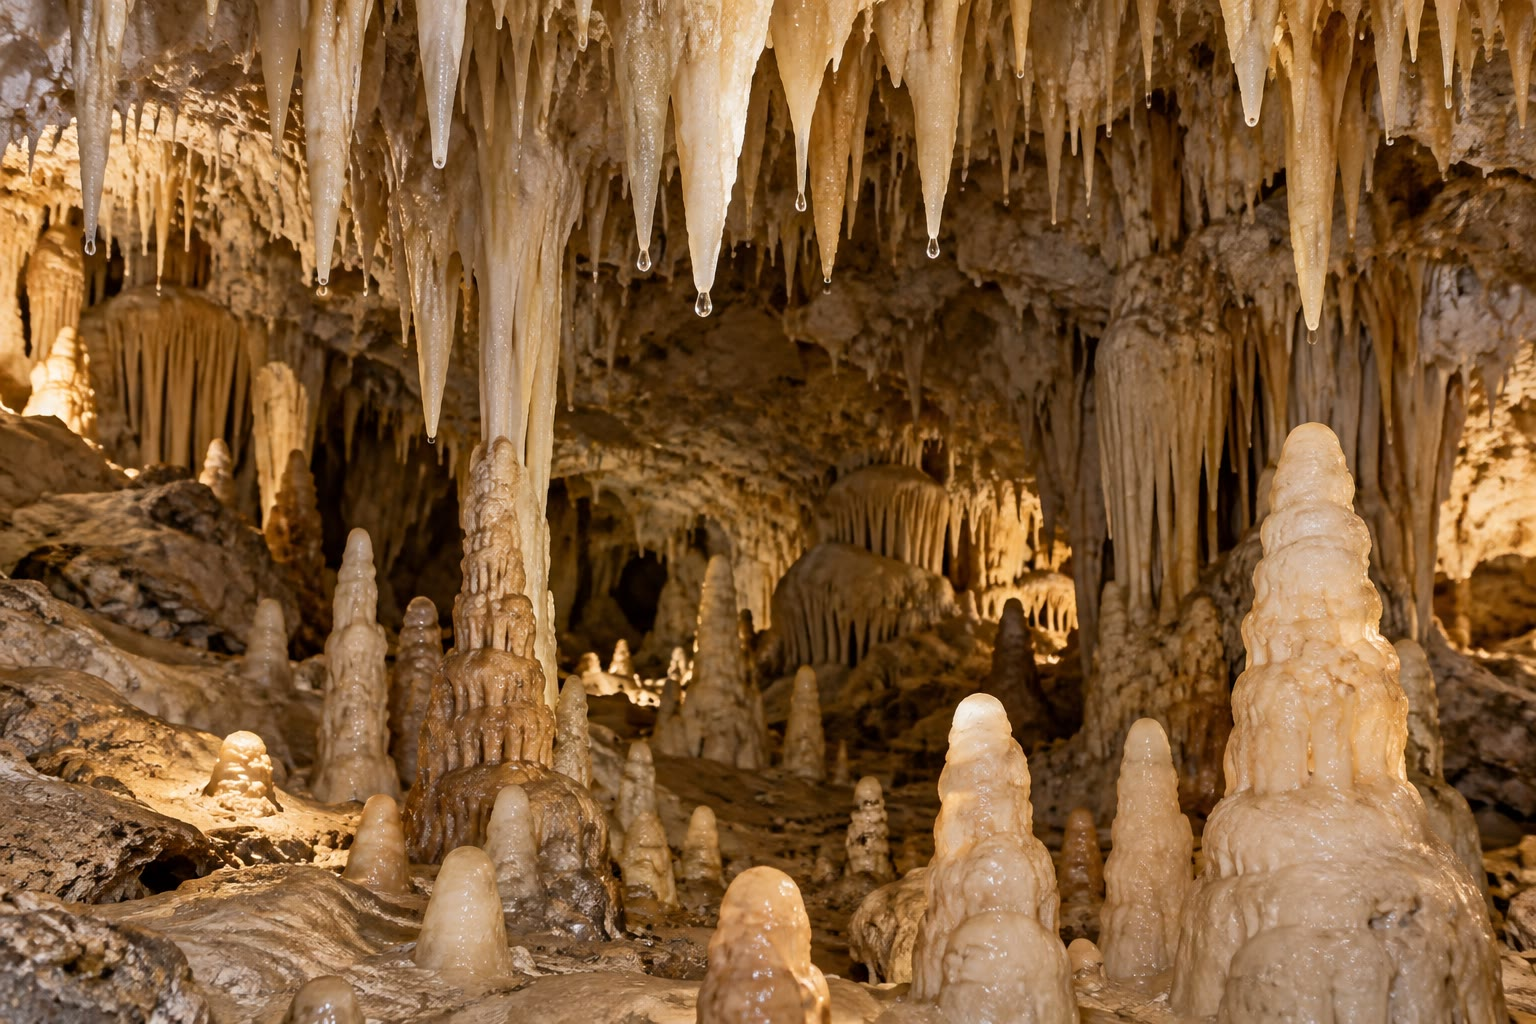
\includegraphics[width=0.45\linewidth]{images/book1/ai/g12-cave-stalactites.jpg}

{\small जहाँ गुफा में टपकता पानी \omterm{def:g4:air-a-mixture-of-gases:air}{वायु} को कार्बन
डाइऑक्साइड खो देता है, वहाँ आश्चुताश्म बढ़ते हैं: घुले हुए चूना-पत्थर का एक साम्य खिसकता है, और
कैल्सियम कार्बोनेट जमा होता है।}
\end{omfigure}

\section{अभ्यास}

\begin{exercise}[$\star$]\label{exo:g12:equilibrium:1}
इनका \omterm{def:g12:equilibrium:quotient}{अभिक्रिया भागफल} लिखिए: (a) \ce{N2 + 3H2 <=> 2NH3} (गैसें, सांद्रताओं
का उपयोग कीजिए); (b) पानी में \ce{CH3COOH + H2O <=> CH3COO- + H3O+};
(c) \ce{CaCO3(s) <=> Ca^{2+} + CO3^{2-}}; (d) \ce{Fe^{3+} + SCN- <=>
FeSCN^{2+}}।
\end{exercise}

\begin{exercise}[$\star$]\label{exo:g12:equilibrium:2}
एक अभिक्रिया का $x_{\max} = \qty{0.050}{mol}$ है और वह
$x_f = \qty{0.020}{mol}$ तक पहुँचती है। $\tau$ निकालिए। क्या अभिक्रिया पूर्ण है?
\end{exercise}

\begin{exercise}[$\star$]\label{exo:g12:equilibrium:3}
$K = 10$ वाली अभिक्रिया के लिए, यदि $Q = 2$ हो तो \omterm{def:g6:pure-substances-and-mixtures:mixture}{मिश्रण} किस दिशा में विकसित होता है?
यदि $Q = 50$? यदि $Q = 10$?
\end{exercise}

\begin{exercise}[$\star$]\label{exo:g12:equilibrium:4}
समझाइए कि साम्य को ``गतिक'' क्यों कहा जाता है।
\end{exercise}

\begin{exercise}[$\star$]\label{exo:g12:equilibrium:5}
क्या \omterm{def:g12:catalysis:catalyst}{उत्प्रेरक} $K$ बदलता है? साम्य तक पहुँचने में लगने वाला समय? समझाइए।
\end{exercise}

\begin{exercise}[$\star\star$]\label{exo:g12:equilibrium:6}
\qty{2.0}{mol} एथेनोइक अम्ल और \qty{2.0}{mol} एथेनॉल मिलाए जाते हैं
($K = 4$)। चारों स्पीशीज़ की अंतिम मात्राएँ निकालिए।
\end{exercise}

\begin{exercise}[$\star\star$]\label{exo:g12:equilibrium:7}
एक \omterm{def:g6:pure-substances-and-mixtures:mixture}{मिश्रण} में एथेनोइक अम्ल, एथेनॉल, एथिल
एथेनोएट और पानी, हर एक का \qty{0.5}{mol} है। $Q$ निकालिए। वह किस दिशा में विकसित होता है?
\end{exercise}

\begin{exercise}[$\star\star$]\label{exo:g12:equilibrium:8}
दोनों प्रयोगों वाले चित्र की मदद से हर प्रयोग में \qty{20}{h} के बाद
\omterm{def:g11:functional-groups:carboxylic-acid}{एस्टर} की मात्रा पढ़िए। निकाय को कब
साम्य में माना जा सकता है?
\end{exercise}

\begin{exercise}[$\star\star$]\label{exo:g12:equilibrium:9}
\qty{1}{mol} \omterm{def:g11:functional-groups:carboxylic-acid}{एस्टर} और \qty{1}{mol} पानी से शुरू करके (एस्टरीकरण के लिए $K = 4$,
इसलिए जल-अपघटन के लिए $1/4$), अध्याय की विधि से अंतिम
मात्राएँ निकालिए, और एस्टरीकरण वाले प्रयोग से
तुलना कीजिए।
\end{exercise}

\begin{exercise}[$\star\star$]\label{exo:g12:equilibrium:10}
\ce{AgCl(s) <=> Ag+ + Cl-} के भागफल में ठोस क्यों दिखाई नहीं देता?
क्या और ठोस मिलाने से
साम्य खिसकता है?
\end{exercise}

\begin{exercise}[$\star\star$]\label{exo:g12:equilibrium:11}
सोडा-पानी की बंद बोतल में कार्बन डाइऑक्साइड पानी को उसी दर से छोड़ती और उसमें प्रवेश करती है।
साम्य \ce{CO2(aq) <=> CO2(g)} लिखिए और $Q$ और $K$ की मदद से
समझाइए कि बोतल खुलने पर पानी बेदम क्यों हो जाता है।
\end{exercise}

\begin{exercise}[$\star\star\star$]\label{exo:g12:equilibrium:12}
\qty{1}{mol} अम्ल और \qty{1}{mol} \omterm{def:g11:functional-groups:alcohol}{ऐल्कोहॉल} का एस्टरीकरण
साम्य तक पहुँचता है। फिर मौजूद पानी का आधा हटा दिया जाता है। नया $Q$
निकालिए, बताइए कि निकाय किस दिशा में विकसित होता है, और \omterm{def:g11:functional-groups:carboxylic-acid}{एस्टर} की नई
अंतिम मात्रा ज्ञात कीजिए।
\end{exercise}

\begin{exercise}[$\star\star\star$]\label{exo:g12:equilibrium:13}
दिखाइए कि उलटी अभिक्रिया का स्थिरांक $1/K$ है। एथिल एथेनोएट के
जल-अपघटन का स्थिरांक क्या है?
\end{exercise}

\begin{exercise}[$\star\star\star$]\label{exo:g12:equilibrium:14}
एक रसायनज्ञ \qty{1}{mol} अम्ल, \qty{1}{mol} \omterm{def:g11:functional-groups:alcohol}{ऐल्कोहॉल},
\qty{2}{mol} \omterm{def:g11:functional-groups:carboxylic-acid}{एस्टर} और \qty{0.5}{mol} पानी मिलाता है। क्या कुछ होगा?
समझाइए।
\end{exercise}

\begin{exercise}[$\star\star\star$]\label{exo:g12:equilibrium:15}
अम्ल के \qty{95}{\percent} का एस्टरीकरण करने के लिए \omterm{def:g11:functional-groups:alcohol}{ऐल्कोहॉल} की कितनी अधिकता (प्रति \omterm{def:g10:the-mole:amount}{मोल} अम्ल मात्रा)
चाहिए? $\dfrac{0.95^2}{0.05(n - 0.95)} =
4$ हल कीजिए।
\end{exercise}

\section{समस्या: बर्थेलो का एस्टर}

\begin{problem}[{सप्ताहांत समस्या --- जब ऐल्कोहॉल तीन गुनी अधिकता में
डाला जाए तो कितना एस्टर?}]
\label{pb:g12:equilibrium:1}
% ledger: ester:berthelot, aw:C, aw:H, aw:O
एथिल एथेनोएट, जो एक \omterm{def:g6:solutions-and-solubility:solute}{विलायक} और सुगंधकारक है, एथेनोइक अम्ल
और एथेनॉल से बनाया जाता है। 1862 में बर्थेलो और पेआं दे सैं-जिल ने पाया कि
अम्ल और \omterm{def:g11:functional-groups:alcohol}{ऐल्कोहॉल} की समान मात्राओं से अभिक्रिया तब रुक जाती है जब लगभग दो तिहाई
अम्ल अभिक्रिया कर चुका होता है।

\medskip
\noindent\textbf{भाग I --- अभिक्रिया।}
\begin{enumerate}
  \item \omterm{def:g11:organic-skeletons:formulas}{अर्ध-संरचना सूत्रों} के साथ एस्टरीकरण का समीकरण
        लिखिए।
  \item इसे दोहरे तीर से क्यों लिखा जाता है?
  \item मात्राओं में इसका \omterm{def:g12:equilibrium:quotient}{अभिक्रिया भागफल} लिखिए।
  \item \qty{1}{mol} अम्ल और \qty{1}{mol} \omterm{def:g11:functional-groups:alcohol}{ऐल्कोहॉल} से
        $x_{\max}$ क्या है? बर्थेलो के परिणाम से $x_f$ क्या है?
  \item $\tau$ निकालिए।
\end{enumerate}

\medskip
\noindent\textbf{भाग II --- स्थिरांक।}
\begin{enumerate}[resume]
  \item चारों स्पीशीज़ की अंतिम मात्राएँ बताइए।
  \item $K$ निकालिए।
  \item \qty{1}{mol} \omterm{def:g11:functional-groups:carboxylic-acid}{एस्टर} और \qty{1}{mol} पानी से शुरू करके
        बर्थेलो ने एक तिहाई जल-अपघटन पाया। दिखाइए कि यह उसी
        $K$ से मेल खाता है।
  \item दोनों स्थितियों में $K$ एक ही क्यों होना चाहिए?
\end{enumerate}

\medskip
\noindent\textbf{भाग III --- \omterm{def:g11:functional-groups:alcohol}{ऐल्कोहॉल} की तीन गुनी अधिकता।}
\begin{enumerate}[resume]
  \item \qty{1}{mol} अम्ल और \qty{3}{mol} \omterm{def:g11:functional-groups:alcohol}{ऐल्कोहॉल} से
        \omterm{def:g10:reaction-progress-table:extent}{प्रगति सारणी} भरिए।
  \item समीकरण $Q_{eq} = K$ लिखिए और दिखाइए कि यह
        $3x^2 - 16x + 12 = 0$ बन जाता है।
  \item इसे हल कीजिए, और सार्थक मूल रखिए।
  \item अम्ल का कितना भाग एस्टरीकृत होता है?
  \item प्राप्त \omterm{def:g11:functional-groups:carboxylic-acid}{एस्टर} का द्रव्यमान निकालिए।
\end{enumerate}

\medskip
\noindent\textbf{भाग IV --- पानी हटाना।}
\begin{enumerate}[resume]
  \item सम-मोलर साम्य से, पानी बनते ही हटा दिया जाता है।
        $Q$ की मदद से समझाइए कि अभिक्रिया क्यों जारी रहती है।
  \item यदि सारा पानी हटाया जा सके, तो \omterm{def:g10:synthesis-yield:yield}{लब्धि} क्या हो जाएगी?
  \item आम तौर पर अम्ल नहीं, बल्कि \omterm{def:g11:functional-groups:alcohol}{ऐल्कोहॉल} अधिकता में क्यों डाला जाता है? (लागत
        और उत्पादों को अलग करने के बारे में सोचिए।)
  \item क्या \omterm{def:g6:pure-substances-and-mixtures:mixture}{मिश्रण} को गरम करने से \omterm{def:g10:reaction-progress-table:system}{अंतिम अवस्था} बदलती है, या केवल
        उस तक पहुँचने का समय? (एस्टरीकरण लगभग कोई ऊष्मा नहीं देता।)
  \item अंतिम उत्तर बताइए: \omterm{def:g11:functional-groups:alcohol}{ऐल्कोहॉल} की तीन गुनी अधिकता के साथ अम्ल का कितना भाग
        एस्टरीकृत होता है?
\end{enumerate}
\end{problem}
